\chapter{Figures}

% Include one figure
\begin{figure}[H] 
	\centering
	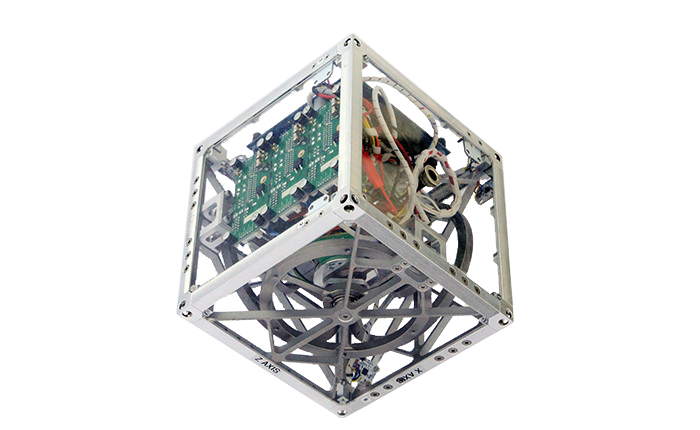
\includegraphics[scale=1.3]{figures/CubliCorner-700x4302}
	\caption{A Cubli balancing on one of its corners.\cite{RAndrea}}
	\label{CubliCorner}
\end{figure}\vspace{-18pt}

% Include to pictures in a row, with different captures
\begin{minipage}{\linewidth}
	\begin{minipage}{0.45\linewidth}
		\begin{figure}[H]
			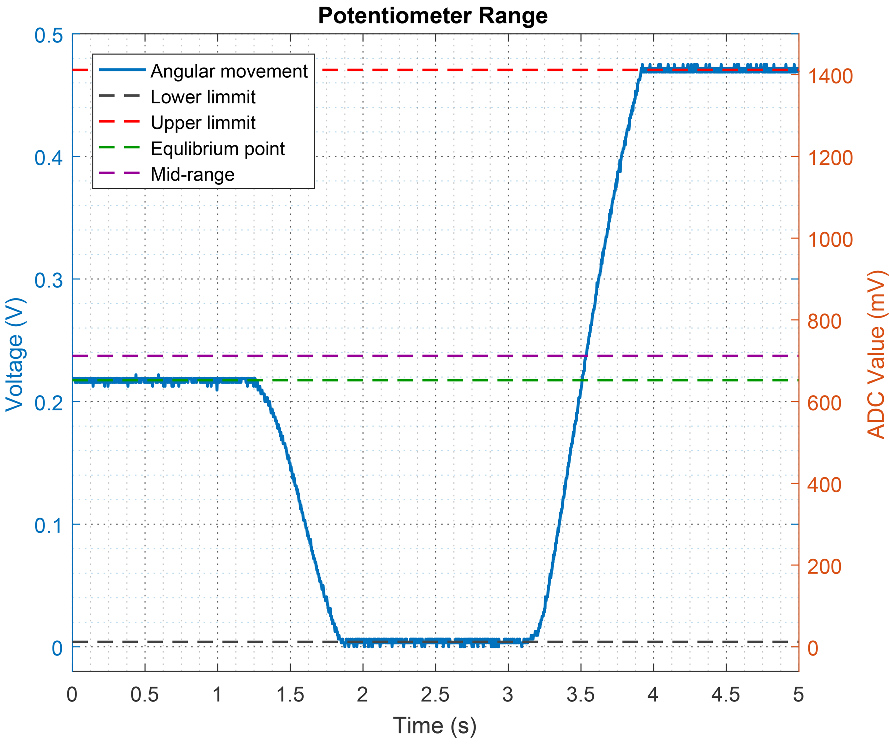
\includegraphics[scale=.5]{figures/PotentiometerResolution}
			\centering
			\captionsetup{justification=centering}
			\captionof{figure}{Potentiometer measurements in volts and the corresponding values that the ADC provides.}
			\label{PotentiometerResolution}
		\end{figure}
	\end{minipage}
	\hspace{0.03\linewidth}
	\begin{minipage}{0.45\linewidth}
		\begin{figure}[H]
			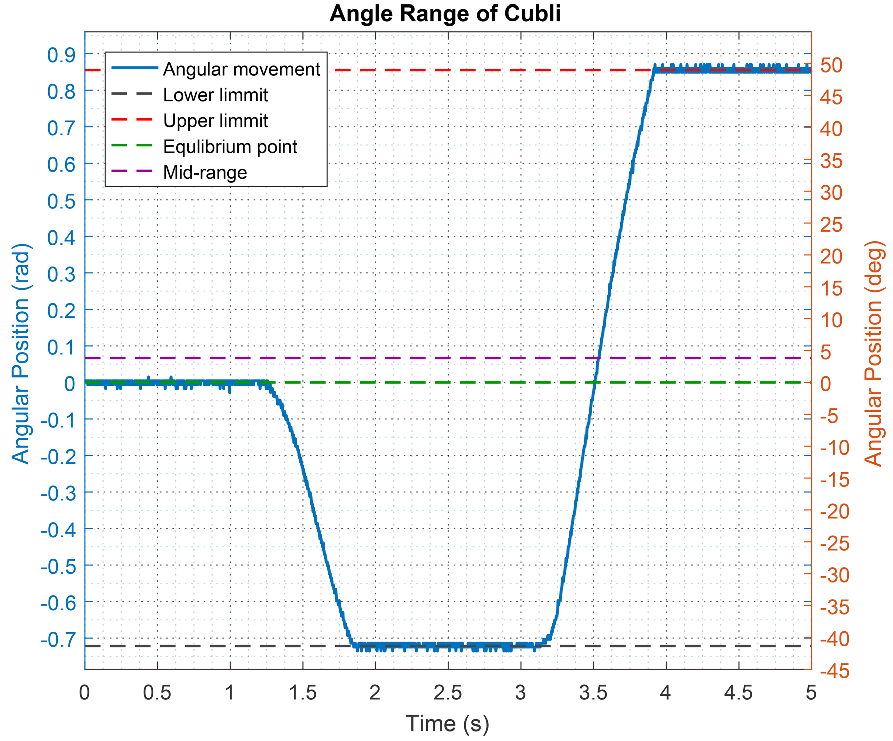
\includegraphics[scale=.5]{figures/PotentiometerResolutionDegRad}
			\centering
			\captionsetup{justification=centering}
			\captionof{figure}{Potentiometer measurements converted to radians and degrees.\vspace{12pt}}
			\label{PotentiometerResolutionRadDeg}
		\end{figure}
	\end{minipage}
\end{minipage}

% Include to pictures in a row, with different captures and a common one
\begin{figure}[H]
	\begin{minipage}{\linewidth}
		\captionsetup[subfigure]{font = footnotesize}
		\centering
		\subcaptionbox
		{
			Here \si{f(x_a) < f(x_b)} resulting in the red interval, \si{x_{L} < x^* < x_a}, and green interval, \si{x_a < x^* < x_b}, which when combined yields the new bracket, \si{[x_{L},\ x_b]}, shown in blue.
			\label{dichotomousLargerB}
		}
		{
			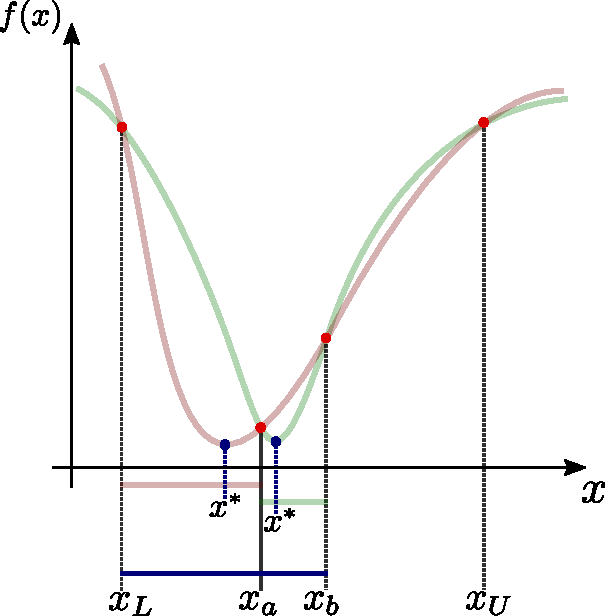
\includegraphics[scale=.6]{dichotomousLargerB}
		}\quad
		\subcaptionbox
		{
			Here \si{f(x_b) < f(x_a)} resulting in the green interval, \si{x_a < x^* < x_b}, and red interval, \si{x_b < x^* < x_{U}}, which when combined yields the new bracket, \si{[x_a,\ x_{U}]}, shown in blue.
			\label{dichotomousLargerA}
		}
		{
			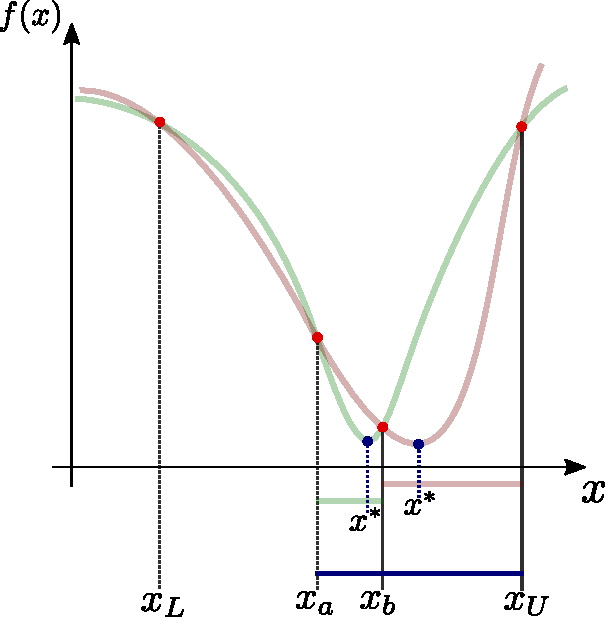
\includegraphics[scale=.6]{dichotomousLargerA}
		}
		\caption{The function, \si{f(x)}, is only evaluated at the points indicated by red dots. Two examples of how the graph of \si{f(x)} could appear is shown in green and red.}
		\label{dichotomousLargerAorB}
	\end{minipage}
\end{figure}\vspace{-18pt}

% Tikz diagrams

\begin{figure}[H]
	  \begin{tikzpicture}[ auto,
                       thick,                         %<--setting line style
                       node distance=1.5cm,             %<--setting default node distance
                       scale=0.75,                     %<--|these two scale the whole thing
                       every node/.style={scale=0.62}, %<  |(always change both)
                       >/.tip={Triangle[angle=40:5pt]}
                       ]

    %-- Blocks creation --%
    \draw
      % DIRECT TERM %
      node[shape=coordinate][](input1) at (0,0){}
      node[shape=coordinate][](feedForward) at (0.5,0){}
      node(sum1) at (7.75,0) [sum] {\si{\sum}}
      node(sum2) at (9.25,0) [sum]{\si{\sum}}
      node(sum3) at (10.75,0) [sum]{\si{\sum}}

      node(torque2rotacc1) at (12.85,0) [block]{\large \si{\frac{1}{J_F + m_w \cdot {l_w}^{2}}}}

      node(integration1) at (15.75,0) [block] {\large \si{\frac{1}{s}}}
      node(integration2) at (18.2,0) [block] {\large \si{\frac{1}{s}}}

      node[shape=coordinate][](output) at (19,0){}
      node[shape=coordinate][](veloFeedbackNode) at (16.8,0){}
      node[shape=coordinate][](accFeedbackNode) at (14.5,0){}
    ;
    \draw
      % REACTION WHEEL EQUATIONS %  
      node(sum4) at (1.5,-1.6) [sum]{\si{\sum}}
      node(sum5) at (2.85,-1.6) [sum]{\si{\sum}}

      node(torque2rotacc2) at (4.3,-1.6) [block]{\large \si{\frac{1}{J_w \cdot s}}}
      % node(integration3) [block, right of = torque2rotacc2] {$\frac{1}{s}$}
      node(frictionWheel) at (6.9,-1.6) [block] {\large $B_w$}

      node[shape=coordinate][](veloWheelFeedback) at (7.75,-3.2){}
    ;
    \draw
      % FEEDBACKS %
      node(accFeedback) at (8, -4.8) [block] {\large \si{J_w}}
      node(veloFeedback) at (12.65,-1.6) [block] {\large \si{B_F}}
      node(angleFeedback) at (11.65,-3.2) [block] {\large \si{(m_F \cdot l_F + m_w \cdot l_w)g}}
    ;
    %-- Block linking --%
    % INPUT %
    \draw[-](input1)        -- node{\large \si{\tau_m(s)}}(feedForward);
    \draw[->](feedForward)  -- (sum1);

    % OUTPUT %
    \draw[-](integration2)  -- (output);
    \draw[->](output)       -- node {\large \si{\theta_{F}(s)}} (20,0);

    % DIRECT TERM %
    \draw[->] (sum1)            -- (sum2);
    \draw[->] (sum2)            -- (sum3);
    \draw[->] (sum3)            -- (torque2rotacc1);
    \draw[->] (torque2rotacc1)  -- node{\large \si{\ddot{\theta}_F(s)}}(integration1);
    \draw[->] (integration1)    -- node{\large \si{\dot{\theta}_F(s)}}(integration2);

    % REACTION WHEEL EQUATIONS %
    \draw[->] (feedForward)     |- (sum4);
    \draw[->] (sum4)            -- (sum5);
    \draw[->] (sum5)            -- (torque2rotacc2);
    \draw[->] (torque2rotacc2)  -- node{\large \si{\dot{\theta}_w(s)}}(frictionWheel);
    % \draw[->] (integration3)    -- (frictionWheel);
    \draw[->] (frictionWheel)   -| (sum1);

    \draw[-] (frictionWheel)       -| (veloWheelFeedback);
    \draw[->] (veloWheelFeedback)  -| (sum5);

    % FEEDBACKS
    \draw[->] (accFeedbackNode)  |- (accFeedback);
    \draw[->] (accFeedback)      -| (sum4);

    \draw[->] (output)           |- (angleFeedback);
    \draw[->] (angleFeedback)    -| (sum2);

    \draw[->] (veloFeedbackNode) |- (veloFeedback);
    \draw[->] (veloFeedback)     -| (sum3);

    %-- Nodes --%
    \draw%--------------------------------------------------------------
      node at (input1)            [shift={(-0.04, -0.05 )}] {\large \textopenbullet}
      node at (output)            [shift={( 0.007, -0.05 )}] {\large \textbullet}
      node at (veloFeedbackNode)  [shift={( 0.007, -0.05 )}] {\large \textbullet}
      node at (accFeedbackNode)   [shift={( 0.007, -0.05 )}] {\large \textbullet}
      node at (feedForward)       [shift={( 0.007, -0.05 )}] {\large \textbullet}
      node at (frictionWheel)     [shift={( 1.025, -0.04 )}] {\large \textbullet}
    ;

    %-- Summation signs --%
      \draw%--------------------------------------------------------------
      node at (sum1) [right = -6.6mm, below = .6mm] {$-$}
      node at (sum1) [right = -3mm, below = 3.9mm]  {$+$} 
      node at (sum2) [right = -6.6mm, below = .6mm] {$+$}
      node at (sum2) [right = -3mm, below = 3.9mm]  {$+$}
      node at (sum3) [right = -6.6mm, below = .6mm] {$+$}
      node at (sum3) [right = -3mm, below = 3.9mm]  {$-$}
      node at (sum4) [right = -6.6mm, below = .6mm] {$+$}
      node at (sum4) [right = -3mm, below = 3.9mm]  {$-$}
      node at (sum5) [right = -6.6mm, below = .6mm] {$+$}
      node at (sum5) [right = -3mm, below = 3.9mm]  {$-$}
    ;

  \end{tikzpicture}
	\caption{Block diagram of the Cubli as a SISO system. The input is the torque applied to the wheel. The output is the angular position of the frame.}
	\label{cubliSimulink}
\end{figure}

\begin{figure}[H]
	\begin{tikzpicture}[ auto,
thick,                         %<--setting line style
node distance=1.5cm,             %<--setting default node distance
scale=0.75,                     %<--|these two scale the whole thing
every node/.style={scale=0.62}, %<  |(always change both)
>=triangle 45 ]

%-- Blocks creation --%
\draw
% DIRECT TERM %
node[shape=coordinate][](input1) at (0,0){}
node[shape=coordinate][](feed) at (0.5,0){}
node(sum1) at (2,0) [sum] {$\sum$}
node(controller) at (4,0) [block]{\Large $D(s)$}
node(plant) at (6,0) [block]{\Large $G(s)$}
node[shape=coordinate][](DummyNode) at (5,-1.5){}
node[shape=coordinate][](FeedbackNode) at (7.5,0){}
;

%-- Block linking --%
% INPUT %
\draw[-](input1)        -- node{\Large $U(s)$}(feed);
\draw[->](feed)  -- (sum1);

% OUTPUT %
\draw[-](plant)  -- (FeedbackNode);
\draw[->](FeedbackNode)       -- node {\Large $Y(s)$} (9,0);

% DIRECT TERM %
\draw[->] (sum1)            -- (controller);
\draw[->] (controller)       -- (plant);

% FEEDBACKS %
\draw[-] (FeedbackNode)  |- (DummyNode);
\draw[->] (DummyNode)  -| (sum1);

%-- Nodes --%
\draw%--------------------------------------------------------------
node at (input1)            [shift={(-0.04, -0.05 )}] {\Large \textopenbullet}
node at (FeedbackNode)      [shift={(0, -0.07 )}] {\Large \textbullet}
;
%-- Summation signs --%
\draw%--------------------------------------------------------------
node at (sum1) [right = -6.6mm, below = .6mm] {$+$}
node at (sum1) [right = -3mm, below = 3.9mm]  {$-$}
;

\end{tikzpicture} 
	\centering
	\caption{Block diagram of the final controlled system.}
	\label{blockDiagramController}
\end{figure}\vspace{-18pt}